\documentclass[11pt]{article}
\usepackage[a4paper,left=1.5cm,right=1.5cm,top=1.5cm,bottom=1.5cm]{geometry}
\usepackage{fancyhdr}
\usepackage{mleftright}
\usepackage{verbatim}
\renewcommand{\headrulewidth}{1pt}
\fancyhead[C]{\textsc{[LINMA2380] --- Homework 4}}
\fancyhead[L]{14 December 2020}
\fancyhead[R]{Group 02}

\usepackage[T1]{fontenc}
\usepackage[utf8]{inputenc}
\usepackage[english]{babel}
\usepackage{graphicx}
\usepackage{subcaption}
\usepackage{csquotes}
\usepackage{mathtools,amssymb,amsthm}
\usepackage[binary-units=true,separate-uncertainty = true,multi-part-units=single]{siunitx}
\usepackage{float}
\usepackage[linktoc=all]{hyperref}
\hypersetup{breaklinks=true}
\graphicspath{{img/}}
\usepackage{caption}
\usepackage{textcomp}
\usepackage{array}
\usepackage{color}
\usepackage{tabularx,booktabs}
\usepackage{titlesec}
\pagestyle{fancy}
\usepackage{mathrsfs}
\usepackage{bm}
\usepackage[ruled,linesnumbered]{algorithm2e}
\usepackage{tikz}
\usetikzlibrary{matrix}
\usetikzlibrary{calc}
\usetikzlibrary{fit}

\DeclarePairedDelimiterX{\norm}[1]{\lVert}{\rVert}{#1}

\newcommand\bovermat[2]{%
  \makebox[0pt][l]{$\smash{\overbrace{\phantom{%
    \begin{matrix}#2\end{matrix}}}^{\text{#1}}}$}#2}
    
\newcommand{\imag}{\mathrm{i}\mkern1mu} % Imaginary unit
\newcommand{\abs}[1]{\left\lvert#1\right\lvert}
\newcommand{\kp}{\otimes}
\DeclareMathOperator{\vect}{vec}

\DeclareMathOperator*{\argmin}{arg\,min}

\DeclareMathOperator{\rank}{rank}
\DeclareMathOperator{\Ker}{Ker}
\DeclareMathOperator{\newdiff}{d} % use \dif instead
\newcommand{\dif}{\newdiff\!}
\newcommand{\e}{\mathrm{e}}
\newcommand{\bo}{\mathcal{O}}

\DeclareMathOperator{\diag}{diag}

\newcommand{\field}{\mathbb{F}} % field
\newcommand{\real}{\mathbb{R}} % real numbers
\newcommand{\complex}{\mathbb{C}} % complex numbers

\newcommand{\snorm}[1]{\norm{#1}_2} % spectral norm
\newcommand{\fnorm}[1]{\norm{#1}_F} % frobenius norm

\setcounter{MaxMatrixCols}{15}

\newcommand\undermat[2]{% http://tex.stackexchange.com/a/102468/5764
	\makebox[0pt][l]{$\smash{\underbrace{\phantom{%
					\begin{matrix}#2\end{matrix}}}_{\text{$#1$}}}$}#2}

\begin{document}
\section*{Exercise A: Minimal polynomial and Smith normal form}
\subsection*{A1}

\subsection*{A2}
We now prove that for all $k\in\{1,...,n\}$, $\delta_k(P(\lambda))=\Pi^k_{i=1}d_i(\lambda)$ where $d_i(\lambda)$ are the diagonal entries of $D(\lambda)$ and $M(\lambda)D(\lambda)N(\lambda)$ is a Smith decomposition of $P(\lambda)$.
\begin{proof}
From A1, we know that $\delta_k(P(\lambda))=\delta_k(D(\lambda))$ and therefore we will consider $\delta_k(D(\lambda))$.\\
We first note that all sub-matrices of $D(\lambda)$ are either triangular inferior, triangular superior or null. The determinants of these sub-matrices are hence given by the product of the diagonal elements. The only sub-matrices for which the determinant is non-zero are these where the indices of the removed rows are identical to the indices of the removed columns. Because 0 has infinitely many divisors, we should therefore only consider the case where this specific case.\\
We denote by $\textbf{j}=(j_1,...,j_k)$, where $j_1<...<j_k$, the indices of the rows and columns that are kept. The determinant associated to $\textbf{j}$ can be written as:
\begin{equation*}
    \det D_{\textbf{j}}(\lambda)=d_{j_1}(\lambda)...d_{j_k}(\lambda)
\end{equation*}
We now use the property that $d_i(\lambda)$ divides $d_{i+1}(\lambda)$ for all $i\in\{1,...,n-1\}$.\\
If we consider the $i$th factor $d_{j_i}(\lambda)$, we observe that $d_i(\lambda)$ divides $d_{j_i}(\lambda)$ as $j_i$ is either equal to $i$ or larger than $i$ (due to the strict inequality $j_1<...<j_k$). Hence $d_{j_i}(\lambda)$ can be rewritten as $a_{j_i}(\lambda)d_i(\lambda)$ for a certain $a_{j_i}(\lambda)\in\complex[\lambda]$. The determinant can thus be developed as:
\begin{equation}\label{detDj}
    \det D_{\textbf{j}}(\lambda)=a_{j_1}(\lambda) d_1(\lambda)...a_{j_k}(\lambda)d_{k}(\lambda)
\end{equation}
We also observe that when $\textbf{j}=(1,...,k)$, we have:
\begin{equation}\label{123}
    \det D_{\textbf{j}}(\lambda)=\Pi_{i=1}^k d_i(\lambda)
\end{equation}
which is a monic polynomial as it is the product of monic polynomials.\\
Because $\Pi_{i=1}^k d_i(\lambda)$ is a divisor of \eqref{detDj} for any $\textbf{j}$ and that $\delta_k(D(\lambda))$ cannot contain any additional factor due to \eqref{123}, we conclude that the monic greatest common divisor of all k-minors of $D(\lambda)$ is $\Pi_{i=1}^k d_i(\lambda)$. Therefore, we have:
\begin{equation}\label{A21}
    \delta_k(P(\lambda))=\delta_k(D(\lambda))=\Pi_{i=1}^k d_i(\lambda)
\end{equation}
\end{proof}
The diagonal entries $d_1(\lambda),...,d_n(\lambda)$ of $D(\lambda)$ are unique and depend only on the sequence $\delta_1(P(\lambda))$,...,$\delta_n(P(\lambda))$.
\begin{proof}
We first consider the first entry $d_1(\lambda)$. From \eqref{A21}, we know that $d_1(\lambda)=\delta_1(\lambda)$. The notion of monic greatest common divisor leads to the unicity of $\delta_1(\lambda)$ and hence we deduce $d_1(\lambda)$ is unique as well. This constitutes the base case of the induction proof.\\
%Next, we show that if $d_1(\lambda)$ is unique then $d_2(\lambda)$ is unique as well. From \eqref{A21}, we have $d_2(\lambda)=\delta_2(\lambda)/d_1(\lambda)$. This implies $d_2(\lambda)$ is unique as the notion of monic greatest common divisor implies the unicity of $\delta_2(\lambda)$ and $d_1(\lambda)$ is unique.
Next, we prove that if $d_k(\lambda)$ is unique then $d_{k+1}(\lambda)$ is also unique. Again from \eqref{A21}, we have that $d_{k+1}(\lambda)=\delta_{k+1}(P(\lambda))/d_k(\lambda)$. By the unicity of the notion of monic greatest common divisor and the unicity $d_k(\lambda)$, we conclude that $d_{k+1}(P(\lambda))$ is unique.\\
Clearly the diagonal entries $d_1(\lambda),...,d_n(\lambda)$ can be computed using the sequence $\delta_1(P(\lambda)),...,\delta_n(P(\lambda))$. First, we have $d_1(\lambda)=\delta_1(P(\lambda))$ and then we use $d_{k+1}(\lambda)=\delta_{k+1}(P(\lambda))/ d_k(\lambda)$ for the next entries.
\end{proof}
There are unimodular matrices $M(\lambda),N(\lambda)\in\complex^{n\times n}[\lambda]$ such that $Q(\lambda)=M(\lambda)P(\lambda)N(\lambda)$ if and only if $\delta_k(P(\lambda))=\delta_k(Q(\lambda))$ for all $k\in\{1,...,n\}$.
\begin{proof}
$\Rightarrow$ This was shown in A1.\\
$\Leftarrow$
From the previous proved statement we know that the diagonal entries of $D(\lambda)$ of the Smith decomposition of $P(\lambda)$ are unique and depend only on the sequence $\delta_1(P(\lambda)),...,\delta_n(P(\lambda))$. As this sequence is the same for $P(\lambda)$ and $Q(\lambda)$, we deduce $D(\lambda)$ is the same for their Smith decompositions:
% does the smith decomposition exist for every matrix ?
\begin{align*}
    P(\lambda)&=M_1(\lambda) D(\lambda) N_1(\lambda)\\
    Q(\lambda)&=M_2(\lambda) D(\lambda) N_2(\lambda)
\end{align*}
where $M_1(\lambda),M_1(\lambda),M_1(\lambda),M_1(\lambda)\in\complex^{n\times n}[\lambda]$ are unimodular and $D(\lambda)\in\complex^{n\times n}[\lambda]$ diagonal.\\
From the first equation, we can write $D(\lambda)=M_1(\lambda)^{-1} P(\lambda) N_1(\lambda)^{-1}$ as $M_1(\lambda)$ and $N_1(\lambda)$ are unimodular and hence invertible. Next, we inject this expression of $D(\lambda)$ in the second equation and we obtain:
\begin{equation*}
    Q(\lambda)=M_2(\lambda) M_1(\lambda)^{-1} P(\lambda) N_1(\lambda)^{-1} N_2(\lambda)
\end{equation*}
Finally, as the inverse of a unimodular matrix is unimodular and the product of unimodular matrices is unimodular, we have $M(\lambda)=M_2(\lambda) M_1(\lambda)^{-1}$ and $N(\lambda)=N_1(\lambda)^{-1} N_2(\lambda)$ which are unimodular matrices such that $Q(\lambda)=M(\lambda)P(\lambda)N(\lambda)$.

\end{proof}

\subsection*{A3}
Let $A\in \complex^{n\times n}$ be a Jordan block with eigenvalue $\lambda_1$. The elementary polynomials of $\lambda I-A$ are equal to: $d_i(\lambda)=1$ for $i=1,...,n-1$ and $d_n(\lambda)=(\lambda-\lambda_1)^n$.
\begin{proof}
We first write the matrix $\lambda I-A$ that we call $P(\lambda)$:
\begin{equation*}
    P(\lambda)=\lambda I-A=
    \begin{pmatrix}
    \lambda-\lambda_1 & -1 & & \\
    & \ddots & \ddots & \\
    & & \ddots & -1\\
    & & & \lambda-\lambda_1 \\
    \end{pmatrix}
\end{equation*}
As we have seen the sequence $d_1(\lambda),...,d_n(\lambda)$ can be derived by the sequence $\delta_1(P(\lambda)),...,\delta_n(P(\lambda))$, we first derive the latter sequence. When computing each $\delta_k(P(\lambda))$, we observe that for $k<n$, a valid sub-matrix to take into account is the one which has all the $-1$ entries on its diagonal. We illustrate here the case where $k=n-1$:
\[P(\lambda) = 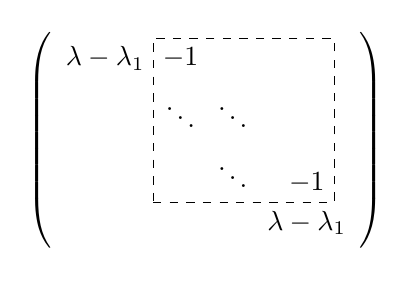
\begin{tikzpicture}[baseline=(math-axis),every right delimiter/.style={xshift=-3pt},every left delimiter/.style={xshift=3pt}]%
\matrix [matrix of math nodes,left delimiter=(,right delimiter=)] (matrix)
{
|(m11)| \lambda-\lambda_1 & |(m12)| -1 & |(m13)| & |(m14)|\\
|(m21)| & |(m22)| \ddots & |(m23)| \ddots & |(m24)| \\
|(m31)| & |(m32)| & |(m33)| \ddots & |(m34)| -1\\
|(m41)| & |(m42)| & |(m43)| & |(m44)| \lambda-\lambda_1\\
};
\node[draw,dashed,inner sep=0pt,fit=(m12) (m14) (m32) (m34)] {};
\coordinate (math-axis) at ($(matrix.center)+(0em,-0.25em)$);
\end{tikzpicture}\]
As this sub-matrix is triangular inferior, its determinant is equal to the product of its diagonal entries. The determinant of such matrices is therefore 1 or -1. As 1 and -1 have only one monic divisor which is 1, we conclude that $\delta_k(P(\lambda))=1$ for $k\in\{1,...,n-1\}$. From the recursive formula proposed in A2, we deduce that $d_k(\lambda)=1$ for $k\in\{1,...,n-1\}$.\\
When $k=n$, the only possible sub-matrix to consider is the whole matrix which determinant is equal to the product of the diagonal entries, hence $(\lambda-\lambda_1)^n$. We deduce that $\delta_n(P(\lambda))=(\lambda-\lambda_1)^n$ and therefore using the recursive formula proposed in A2 we obtain $d_n(\lambda)=(\lambda-\lambda_1)^n$.
\end{proof}

\subsection*{A4}

\subsection*{A5}

\section*{Exercise B: Implementation}
\subsection*{B1}
Using the Jordan normal form is not numerically stable because taking limits does not commute with forming the Jordan canonical form.
A simple example is the matrix \(A = I_2\), approximated by \(A_\varepsilon = \left[\begin{smallmatrix} 1 & \varepsilon \\ 0 & 1\end{smallmatrix}\right]\), the latter having Jordan canonical form \(J_\varepsilon = \left[\begin{smallmatrix} 1 & 1 \\ 0 & 1\end{smallmatrix}\right]\).
However, the Jordan form of \(A\) is simply \(J = I_2\).
We thus have
\[
\lim_{\varepsilon \to 0} A_\varepsilon = A, \quad \textnormal{but} \quad \lim_{\varepsilon \to 0} J_\varepsilon \neq J.
\]
Similarly, computing the minimal polynomials yields \(p_{A_\varepsilon}(\lambda) = (\lambda - 1)^2 \ne \lambda - 1 = p_A(\lambda)\).

\subsection*{B2}

\end{document}